\cotefile{29}
\scanpage{36}
as developped in Exp VI, and under a mild restriction \inserted{in the nature} of a \unsure{connectedness} assumption, we \unsure{can|cpn} say that the category in question is \deleted{\unsure{classifind|classified}} completely described by a certain pro-finite group, the so-called fundamental group of $(Z,G)$, which in fact is an extension of $G$ by the usual fundamental group of $Z$. On the other hand, for these latter considerations, all normality assumptions are completely superflu\deleted{s}ous. Their main use was to insure that the functor $Z'\quad Z'/G$ from étale coverings of $(Z,G)$ to coverings of $S$ is fully faithful; this latter fact, on the other hand, reduces at once to the case when $Z$ is a principal covering of $S$, with group $G$ (\unsure{because|befause} this condition will be satisfied when restricting to a non empty open set $U$ of $S$, and on the pther hand the restriction functors \deleted{fr} to $U$ resp. $Z/U$ are fully faithful, because of normality); but in this case descent theory tells us that we get in fact an \uline{equivalence} of the category of \uline{étale} coverings of $S$, and the catégory of étale coverings of $(Z,G)$ !

In most applications however, instead of having just one model for ramification (one $Z_a^n$ say), we have an infinity of such (all $Z_a^n$ say, \unsure{fixed} $a$ and variable $n$), and the condition on coverings \inserted{$S'$} of $S$ we are \unsure{interested} in is that the covering should (at least locally) have ramification no \unsure{wosse|worse} than one of the $Z_i$ . This situation is described in example twp, On the other hand, sometimes the ramification models are not defined globally (for instance in the Kummer case, when we give \deleted{ideals which \unsure{ar|as}} divisors which are not principal), only locally, in a way that among the set of \unsure{models|modals} given over various open sets (or more generally, objects \unsure{of} the étale site) there are certain compatibility conditions, roughly that the restriction of any model over $U$ to $U\;V$ has ramification no \unsure{worse} than the restriction of some model given over $V$. Such an example is
% archive sheet number: 35

\scanpage{37}
dealt with in example 3, which has the disadvantage of being somewhat involved and artificial in its technical details, but has the merit of allowing explicit construction of the functor ``geometric realization''. Otherwise, the set up outlined before the examples seems more natural, and giving a closer grasp of the \deleted{\unsure{main}} really essential features of what ``ramification data'' should really mean.(By the way, one shoul rather say ``category of ramification data'').

You are of course right that in the definition of a Galois covering when I \unsure{wssume|assume} that the \unsure{soverings|coverings} of the various $\underline{s}(M)$ are Galois étale coverings with Galois group $G$, that beforhand an action of $\unsure{E|G}$ on $X$ was given, which means that $G$ acts on each of the coverings $X(M)$ of $\underline{s}(M)$ on a way compatible with the base changes $\underline{s}(M')\quad\underline{s}(M)$ stemming from arrows \deleted{along the} $M'\quad M$. In the various examples 1 to 3, this means that the action of $G$ commutes to \inserted{étale} localization on $S$ (i.e. base changes $\unsure{S''|S'}\quad S'$\deleted{\unsure{on} $S$} in the étale site of $S$) \uline{and} to the action of the groups of automorphisms given on the various $Z$'s .

Now let's come back to the case $S$ strictly local; then (for coverings defined over t he whole of $S$) the general situation of example 3 reduces to the one of example 2, and replacing the $Z_i$'s by suitable connected components, we may assume them connected if we want. For a given $\unsure{Z_i|Z_i'}$, the $\deleted{f_i}$ étale coverings of $(Z_i,G_i)\deleted{\unsure{x|,}}$ are trivial as coverings of $Z_i$ alone (i.e. forgetting the action of $G_i$) be\deleted{\unsure{r|x}}cause $Z_i$ is strictly local too. Therefore the catégory of étale coverings of$(Z_i\inserted{,G_i)}$ is just equivalent to the category of finite sets $E$ on which $G_i$ opérates; to such an $E$ is associated the consatnt covering $E_{Z_i}$ of $Z_i$, \unsure{byt|but} $G_i$ operating on it via it's operation on $E$; the geometric relaization over $S$ of this is nothing else but $Z_i\overset{G}{x}E$ , the \unsure{vovering|covering} associated to the $G$-covering
% archive sheet number: 36

\scanpage{38}
$Z_i$ of $S$ and the action of $G_i$ on $E$.\inserted{When $S$ is again arbitrary,}This shows in a \unsure{rather|rahher} concrete way what it means, \inserted{locally(for étale topology)} for a covering $S'$ of $S$, to be associated to some $M$: it means that locally it is describable by a representation of an inertia\deleted{l} group on a finite set, in the obvious way; and the extra structure on one $S'$ involved by deducing it from some $S$, can be described by saying that we give such local representations of $S'$, in such a way that they match together i.e. satisfy some rather evident compatibility condition (This description makes a sense whenever the functor ``\unsure{geometri} realization'' is faithful - not necessarily fully faithful). The analogous description holds for Galois coverings with Galois group $\unsure{G|H}$, namely in the strictly local case, for a fixed $Z_i$ , the\deleted{y are classified by systems (} category of these is equivalent to the category of finite sets $E$ on which $G_i$ operates on the left, $H$ on the right, $G_i$ and $H$ commuting, in such a way that $E$ is a principal homogeneous space (or, as we say, a torsor) under $H$; up to isomorphism, they are classified by $\operatorname{Hom}(G_i,H)/H$ , group homomorphisms mod. interior automorphism. Using \deleted{th} this description, one easily proves the criterion I indicated for the ``geometric\deleted{\unsure{-|r}}re\unsure{l|a}\unsure{l|a}ization -functor'' to be fully faithful on the category of \unsure{\c{\u{G}}}alois coverings of type $\underline{R}$ ; indeed, as usual the question is a \unsure{pocal|local} one for the étale topology, which allows one to \deleted{restr} reduce to\unsure{'} the stricly local case.

Your interpretation of the Kummer case in the final \unsure{s|f}\unsure{o|i}rmulation of example 3 is indeed the one I had in \unsure{mihd|mind}. Also, when I wrote $n'\quad n$, I meant of course the order relation of divisibility (it may be convevient to introduce this order relation explicitly, for simplicity of notations).
% archive sheet number: 37

\scanpage{39}

I realize that all the indications I have given you so far are extremely sketshy, and as a consequence that I am charging you with a considerable amount of work to put some sense and order into all that. Thus it is I, not you, who should apologize for causing a lot of trouble! I look forward with great pl\unsure{a|e}\unsure{d|a}sure meeting you in Bures. As I am having some russian andchinese lessons on fridays, I will probably drop by on June 2.

With best regards\\

% Isolated ochre mark far below the closing: shape retained; material, maker,
% and deliberate/accidental status unresolved. No readable letters asserted.
\figure{
\begin{tikzpicture}[x=1mm,y=1mm]
\path[fill=brown!65!orange,draw=none]
 (0,2.85) .. controls (.22,2.9) and (.35,2.8) .. (.51,2.84)
 .. controls (.69,2.97) and (.89,2.86) .. (1,2.84)
 -- (1.07,3.08) .. controls (1.25,2.8) and (1.3,2.43) .. (1.36,2.18)
 .. controls (1.5,1.69) and (1.7,1.24) .. (1.82,.74)
 .. controls (1.99,.38) and (1.91,.13) .. (1.77,.1)
 -- (1.3,.07) -- (.98,0) .. controls (.6,.11) and (.45,.34) .. (.37,.77)
 .. controls (.21,1.34) and (.2,1.78) .. (.13,2.15) -- cycle;
\draw[line width=.24mm,brown!55!black,line cap=round]
 (.06,2.83) .. controls (.16,2.42) and (.36,1.98) .. (.57,1.53)
 .. controls (.71,1.13) and (.83,.67) .. (.97,.24)
 .. controls (1.06,.07) and (1.3,.12) .. (1.32,.24);
\draw[line width=.2mm,brown!55!black,line cap=round]
 (.59,2.81) .. controls (.72,2.42) and (.89,2.1) .. (1.03,1.72)
 .. controls (1.21,1.35) and (1.4,.97) .. (1.6,.7);
\draw[line width=.17mm,brown!55!black,line cap=round]
 (1.08,3.03) .. controls (1.15,2.6) and (1.25,2.2) .. (1.36,1.85)
 .. controls (1.56,1.23) and (1.77,.6) .. (1.76,.13);
\draw[line width=.17mm,brown!55!black,line cap=round]
 (.3,1.2) .. controls (.25,.72) and (.46,.35) .. (.76,.2);
\end{tikzpicture}}

% archive sheet number: 38

\scanpage{83}
\mspage{\handwritten{74}}
% One long diagonal cancellation crosses the main text of the sheet.
\deleted{ment constant à fibres finies et que les ${}_nG^{\unsure{o|0|\circ}}$ (pour $n\handwritten{\geq}1$) sont des schémas en groupes \deleted{\unsure{les}} finis localement libres sur $S$, que $H$ est fini localement libre sur $S$, et que \handwritten{l}a formation \deleted{commute} de $\underline{\operatorname{Hom}}(\underline{\unsure{\varnothing|\phi|\Phi}}\ ,\ G^{\handwritten{o\natural}})$ commute à\handwritten{\textsubscript{q}} tout changement de base. Appliquant les mêmes réflexions aux extensions de $\underline{\varnothing}_n$ par $G^o_n$ , on trouve que celles-ci correspondent aux torseurs sous le Groupe $H_n=Hx_SS_n\handwritten{\simeq}\underline{\operatorname{Hom}}(\underline{\varnothing}_n,\ G^o_n)$. Or, $H$ étant fini localement libre sur $S$, on en conclut aussitôt que la \deleted{donnée du} catégorie des torseurs \inserted{$P$} sous $H$ équivaut (par le foncteur ``complétion formelle'') à la catégorie des torseurs sous $\overset{\unsure{\scriptscriptstyle\wedge}}{H}$ i.e. des``systêmes cohérents'' de torseurs $P_n$ sous les $H_n$ . Cela implique donc que la catégorie des extensions de $\underline{\varnothing}$ par $G^{o\handwritten{\natural}}$ équivaut à celle des \deleted{extensions de} ``systêmes cphérents'' d'extensions des $\underline{\varnothing}_n$ par les $G^o_n$ , ce qui précise donc la définition de l'extension $G^{\handwritten{\natural}}$ de (7.6.1).}

\deleted{Le schéma en groupes $G^{\handwritten{\natural}}$ , en tant qu'extension de $\underline{\varnothing}$ par $G^{o\handwritten{\natural}}$ , dé\deleted{\uline{p\unsure{e}}}pend évidemment encore de façon fonctorielle de $G$. Sa formation est compatible aux changements de base par un morphisme de traits complets $S'\handwritten{\longrightarrow}S$.}

\margin{\handwritten{$\unsure{V|\checkmark}$}}
\deleted{7.6.3.Notons que les constructions \unsure{p|d}\unsure{r|e}écédentes gardent également un sens sur une base plus générale qutun \deleted{trait}\inserted{sbhéma \uline{local}} complet; il suffit de partir d'un anneau noethérien adique $\deleted{\unsure{\mathbb{X}|\mathbb{V}|X}}\handwritten{V}$, dont la topologie est définie par un \deleted{sché} idéal $\underline{m}\handwritten{\subset}\deleted{\mathbb{X}}\handwritten{V}$, et d'un schéma en groupes $G$ sur $\deleted{\mathbb{X}}\handwritten{V}$ tel que $G_{\unsure{o|0}}=G\otimes_{\deleted{\mathbb{X}}\handwritten{V}}\deleted{\mathbb{X}}\handwritten{V}_o$ (où $\deleted{\mathbb{X}}\handwritten{V}_o=\mathbb{X}/\underline{m}$) soit extension d'un schéma en groupes étale fini par un schéma abélien par un \deleted{schéma} tore. La question essentielle est celle de montrer que le schéma formel abélien $\overset{\handwritten{\scriptscriptstyle\wedge}}{B}$\inserted{sur $\deleted{\mathbb{X}}\handwritten{V}$} construit comme dans 7.1 en termes de $G^o$ est algébrisable; cela se voit par la méthode de 7.2 lorsqu'on suppose que $S$ est normal.}
% archive sheet number: 82

\scanpage{102}
\mspage{101}
% Upper-left margin: thin grey curved line; origin unassigned.
\margin{\figure{\begin{tikzpicture}\draw[gray,line width=.2pt] (0,0) .. controls (1,-.13) and (2.2,-.19) .. (3.2,-.14);\end{tikzpicture}}}
% Upper-right margin: two separate diffuse brown-grey traces with darker centres; no textual value or maker assigned.
\margin{\figure{\begin{tikzpicture}
\fill[brown!30!gray,opacity=.45] (-.018,.02) .. controls (.03,.01) and (.04,-.08) .. (.027,-.17) .. controls (-.01,-.20) and (-.04,-.09) .. cycle;
\fill[black!65] (-.012,-.145) .. controls (.015,-.157) and (.023,-.172) .. (.004,-.181) .. controls (-.018,-.178) and (-.024,-.159) .. cycle;
\fill[brown!30!gray,opacity=.45] (.385,-.66) .. controls (.42,-.72) and (.43,-.83) .. (.408,-.96) .. controls (.39,-1.07) and (.36,-1.14) .. (.348,-1.18) .. controls (.326,-1.19) and (.341,-1.08) .. (.365,-.96) .. controls (.39,-.83) and (.36,-.72) .. cycle;
\fill[black!65] (.372,-.90) ellipse (.015 and .018);
\fill[black!65] (.371,-1.01) .. controls (.391,-1.035) and (.376,-1.06) .. (.356,-1.063) .. controls (.348,-1.045) and (.36,-1.02) .. cycle;
\fill[black!45] (.350,-1.10) .. controls (.373,-1.085) and (.371,-1.13) .. (.341,-1.16) .. controls (.335,-1.145) and (.341,-1.12) .. cycle;
\end{tikzpicture}}}

Examinons maintenant le cas où l'un des cycles $\underline{a}$ ou $\underline{b}$ (par exemple $\underline{b}$) appartient au noyau d'Albanese $Z_{\handwritten{\ell}}(A)$ ; par linéarité, on se ramène au cas où $\underline{b}$ est de la forme $\underline{c}_u-\underline{c}$, avec $\underline{c}\handwritten{\in}Z^{s}_{\unsure{o|0}}(A)_{\bar{\underline{k}}}$, et $u\handwritten{\in}{}^{s}A_{\bar{\underline{k}}}$. D'après l'invariance du symbole $j_{\handwritten{o}}$ par la translation $\handwritten{\tau_u}$, les deux membres de (3) sont respectivement égaux à $j_{\handwritten{o}}(Y_{\underline{a}},\underline{c})$ et à $j_{\handwritten{o}}(Y^{-}_{\underline{c}},\underline{a})$\inserted{\handwritten{, en posant $Y=X_u-X$.}} Puisqu'on a $X\handwritten{\in}D_a(A)$, on a $Y\handwritten{\sim}0$, et on est ramené au cas déjà traité.
% The handwritten insertion begins with comma + en at the right end of line 6;
% posant Y=X_u-X. continues in the left margin at line 7, before Puisqu'on.

Supposons maintenant $X$, $\underline{a}$ et $\underline{b}$ quelconques. On peut, en modifiant $\underline{b}$ par l'addition d'un élément de $Z^{\handwritten{s}}_{\handwritten{\ell}}(A)_{\handwritten{\bar{\underline{k}}}}$, se ramener au cas où le cycle $\underline{a}^{-}\handwritten{\otimes}\underline{b}$ est étranger à $X$. Les symboles $X_{\underline{a}}(\underline{b})$ et $X^{-}_{\underline{b}}(\underline{a})$ sont alors définis, et on a
\[
X_{\underline{a}}(\underline{b})=X^{-}_{\underline{b}}(\underline{a}),\quad\text{d'où}\quad v(X_{\underline{a}}(\underline{b}))=v(X^{-}_{\underline{b}}(\underline{a})).
\]

D'autre part, soit $a$ (resp. $b$) l'un quelconque des composants de $\underline{a}$ (resp. $\underline{b}$). Alors les symboles $i(X_a,b)$ et $i(X^{-}_b,a)$ sont définis ; l'application $\handwritten{\unsure{\zeta|\xi}}:A\handwritten{\longrightarrow}A$ définie par $\handwritten{\zeta}(x)=a+b-x$ étant \uline{p}-isomorphique en $b^{\handwritten{\unsure{\circ|o|0}}}$, de valeur $a^{\handwritten{\circ}}$, on a, d'après la propriété d'invariance du symbole $i$,
\[
i(X_a,b)=i(X^{-}_b,a).
\]

Il en résulte, par linéarité,
\[
i(X_{\underline{a}},\underline{b})=i(X^{-}_{\underline{b}},\underline{a}).
\]
% Left margin beside the second i display: gray stem and dark filled lobes; origin unassigned.
\margin{\figure{\begin{tikzpicture}[x=1cm,y=1cm]
\fill[black!35] (0,0) .. controls (-.004,-.04) and (.006,-.08) .. (.018,-.11) .. controls (.023,-.14) and (.020,-.17) .. (.026,-.20) .. controls (.040,-.24) and (.045,-.28) .. (.037,-.30) .. controls (.018,-.31) and (.009,-.27) .. (.013,-.24) .. controls (.020,-.21) and (.022,-.20) .. (.012,-.18) .. controls (.005,-.15) and (.011,-.13) .. (.008,-.10) .. controls (-.003,-.06) and (-.006,-.02) .. (0,0);
\fill[black] (.019,-.12) .. controls (.030,-.14) and (.022,-.17) .. (.026,-.18) .. controls (.008,-.17) and (.008,-.15) .. (.019,-.12);
\fill[black] (.024,-.22) .. controls (.034,-.24) and (.044,-.28) .. (.037,-.30) .. controls (.019,-.31) and (.011,-.28) .. (.013,-.25) .. controls (.014,-.23) and (.019,-.22) .. (.024,-.22);
\end{tikzpicture}}}

Compte tenu des formules (2) précédentes, on en déduit (3).

Notons enfin \unsure{.}que $j_{\handwritten{o}}(X,\underline{a})$ s'annule lorsque tous les composants de $A$ appartiennent au groupe ${}^{s}A_{\bar{\underline{k}},\handwritten{o}}$. En effet, soit $f$ une fonction sur $V$, définie sur $\underline{k}$, telle que

% archive sheet number: 101

\scanpage{113}

\uline{Théorème de Bertini et variantes}.

Dans la suite $k$ désigne un corps, $P^r=P^r_k$.

\margin{\figure{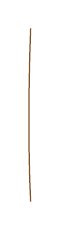
\begin{tikzpicture}\draw[brown!65!black,line width=.45pt] (0,0) .. controls (-.03,-.8) and (-.03,-1.6) .. (0,-2.2);\end{tikzpicture}}}
\uline{Théorème de Bertini} 1: Soit $f:X\handwritten{\rightarrow}P^r_k$ un morphisme, où $X$ est un schéma algébrique géométriquement irréductible, et soit $n=\dim\overset{\handwritten{\rule{1.9em}{.4pt}}}{f(X)}$. Soit $L_t$ le\deleted{\unsure{s|un}} sous-espace linéaire de codimension $s$ \uline{générique} de $P^r$, où $s$ est un entier fixé $\handwritten{\leqslant}n-1$. Alors $\inserted{Y_t=}f_t^{-1}(L_t)\handwritten{\subset}X_t=X\otimes_k k(t)$ est géométriquement irréductible.

\margin{\handwritten{\unsure{vrai} dans\\\unsure{E|S}GA \unsure{V|IV}}\figure{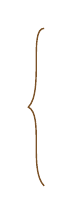
\begin{tikzpicture}\draw[brown!65!black,line width=.5pt] (.2,0) .. controls (0,0) and (.2,-.8) .. (0,-1) .. controls (.2,-1.1) and (0,-1.8) .. (.2,-2);\end{tikzpicture}}}
\margin{\figure{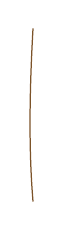
\begin{tikzpicture}\draw[brown!65!black,line width=.45pt] (0,0) .. controls (-.04,-.7) and (-.06,-1.5) .. (0,-2.2);\end{tikzpicture}}}
\inserted{Enoncé local 2: Soit $f:X\handwritten{\rightarrow}P^r$ un morphisme, avec $X$ un schéma algébrique.} \deleted{\uline{Complément}\unsure{:} Supposons} Soit $Z\handwritten{\rightarrow}X$ \deleted{\illegible{2}} l'ensemble des points de $X$ en lesquels \inserted{\handwritten{soit}} $f$ est \deleted{\handwritten{soit}} ramifié \deleted{ou en lesquels} \inserted{\handwritten{soit}} $X$ n'est pas géométriquement unibranche (resp.\ \inserted{\handwritten{pas}} normal, resp.\ \inserted{\handwritten{pas}} lisse \ldots), \deleted{alors} et supposons que $\overset{\handwritten{\rule{1.9em}{.4pt}}}{f(Z)}$ soit de dimension $\handwritten{<}s$. Alors $\inserted{Y_t=}f_t^{-1}(L_t)$ est géométriquement unibranche (resp.\ normal, resp.\ lisse \ldots), où $L_t$ est comme ci-dessus.

De ces deux énoncés on déduit\handwritten{/}formellement;

\margin{\figure{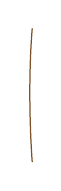
\begin{tikzpicture}\draw[brown!65!black,line width=.45pt] (0,0) .. controls (-.05,-.6) and (-.03,-1.3) .. (0,-1.7);\end{tikzpicture}}}
\deleted{Thé}\uline{Corollaire} 3: Soit $f:X\handwritten{\longrightarrow}P^r$ satisfaisant les conditions de 1\handwritten{,} et 2 non respé.\ \inserted{Supposons $k$ alg.\ clos.} Alors l\unsure{e|'}\deleted{inclusion} morphisme canonique
\[
\handwritten{\pi}_1(Y_{\bar{t}})\handwritten{\rightarrow}\handwritten{\pi}_1(X)
\]
est surjectif.

\uline{Re\unsure{ma}\unsure{r|q}que} \unsure{3|4}. Utilisant les théorèmes de changement de base pour le $\handwritten{\pi}_1$, on conclut \deleted{que} (posant $X_{\bar{t}}=X\otimes_k k(\bar{t})$) que l'homomorphisme $\deleted{\unsure{\pi}_1(}$
% The written display label is at the left margin.
\[
\handwritten{\pi}_1(Y_{\bar{t}})\handwritten{\rightarrow}\handwritten{\pi}_1(X_{\bar{t}})\tag*{\makebox[0pt][r]{\makebox[\linewidth][l]{(*)}}}
\]
est surjectif si $X_{\deleted{\unsure{t|\bar{t}}}}$ est propre, et que l'homomorphisme
% Both X- and Y-like contours occur in the source cell; no correction order is established.
% The written display label is at the left margin.
\[
\handwritten{\pi}_1^{!}(\unsure{X|Y}_{\bar{t}})\handwritten{\rightarrow}\handwritten{\pi}_1^{!}(X_{\bar{t}})\tag*{\makebox[0pt][r]{\makebox[\linewidth][l]{\handwritten{(**)}}}}
\]
est surjectif, où le ! désigne le plus grand quotient profini premier à l'è\unsure{d|x}posant car.\ de $k$. On n'affirme pas, cependant, que (*) soit toujours surjectif (sans hypothèse de propreté sur $X$).

On déduit, de 1, par une application facile du théorème de connexité:

% The second marginal numeral retains the V/IV ambiguity first marked in the upper note.
\margin{\handwritten{vu.\ dans\\EGA V}\figure{\begin{tikzpicture}\draw[brown!65!black,line width=.45pt] (0,0)--(.03,-.5);\end{tikzpicture}}}
\uline{Corollaire} 4 (de 1): Sous les conditions de 1) pour $f:X\handwritten{\longrightarrow}P^r$, si $X$
% archive sheet number: 112

\scanpage{114}
\margin{\figure{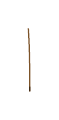
\begin{tikzpicture}
\draw[brown!65!black,line width=.45pt] (0,0) .. controls (.015,-.20) and (.02,-.55) .. (.02,-.80);
\draw[brown!35!black,line width=.45pt] (.019,-.74)--(.02,-.80);
\end{tikzpicture}}}
est de plus propre, alors pour \uline{toute} sous-variété linéaire $\inserted{L_t}$ de codimensio\handwritten{n} $s$, $Y_t=f_t^{-1}(L_t)$ est géométriquement connexe.

Conjuguant avec 2, on trouve, par l'argument qui a permis de déduire 3 de 1 :

\margin{\handwritten{\begin{tabular}{@{}l@{}}cf.\\S\unsure{C|G}A 1 X \unsure{2,11|2.11|2,II|2.II}\end{tabular}}}
\margin{\figure{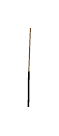
\begin{tikzpicture}\draw[brown!55!black,line width=.35pt] (.025,0)--(.005,-.55);\draw[black,line width=.55pt] (.005,-.55)--(0,-1);\end{tikzpicture}}}
\uline{Corollaire} 5: \deleted{Avec}\inserted{\handwritten{Sous}} les hypothèses de \unsure{3|4} , \inserted{avec $X$ propre,} l'homomorphisme danonique $\handwritten{\pi}_1(Y_{\bar t})\handwritten{\rightarrow}\handwritten{\pi}_1(X)$ ($\handwritten{\simeq}\handwritten{\pi}_1(X_{\bar t})$ par le théorème de changement de base) est surjectif.

Nous désirons également un énoncé analogue à 5, donnant une surjectivité pour des $\handwritten{\pi}_1$ pour un $t$ non générique, mais sans hypothèse de propreté, et pour des quotients plus gros du $\handwritten{\pi}_1$ que ceux envisagés dans (**). On peut\deleted{n\unsure{t|l}} donner à ce sujet le résultat suivant:

\margin{\figure{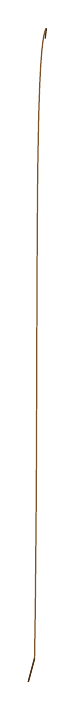
\begin{tikzpicture}
\draw[brown!65!black,line width=.45pt] (.15,0) .. controls (-.02,-.2) and (.06,-4) .. (0,-8) --(-.08,-8.3);
\draw[brown!35!black,line width=.45pt] (.15,0)--(.135,-.13);
\draw[brown!35!black,line width=.45pt] (0,-8)--(-.08,-8.3);
\end{tikzpicture}}}
\uline{Théorème} 6. Su\unsure{p|i}\unsure{p|t}osons $k$ algébriquement clos, \inserted{\handwritten{et}} $X$ propre, $f:X\handwritten{\rightarrow}P^r$, \deleted{et} le sous -espace linéaire $L_t$ de $P^r$ de codimension $s$ (défini sur $k$, pour fixer les idées) \deleted{tels qu'on ait} et enfin le sous-schéma fermé $D$ de $X$ tels qu'on ait ceci; \deleted{où on a posé $U=X-D$}

a) \deleted{$U_t=U\unsure{\cap}X_t$ et} $\deleted{X}\handwritten{Y}_t=f^{-1}(L_t)$ est non vide.

b) Pour tout $x\handwritten{\in}\deleted{X}\handwritten{Y}_t$ , $X$ est lisse en $x$, $Y_t$ est lisse en $x$\handwritten{,} de codime\unsure{m|n}tsion $s$ dans $X$ en $x$, $f$ est net en $x$.

c) Pour tout $x\handwritten{\in}D_t=D\handwritten{\cap}Y_t$ , o\deleted{\unsure{\`{}}}u \deleted{bien} bien $\operatorname{codim}_x(D_t,\mathord{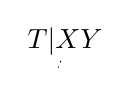
\begin{tikzpicture}[baseline=(g.base),x=1em,y=1em]\node[inner sep=0pt] (g) at (0,0) {$\deleted{\unsure{T|X}}\handwritten{Y}$};\fill[black] (-.17,-.73) ellipse (.026 and .036);\fill[brown!60!black] (-.24,-.92) circle (.03);\end{tikzpicture}}_t)\handwritten{\geqslant}2$, ou bien $D_{\deleted{\unsure{t}}}$ est un diviseur \unsure{e|s}\unsure{n|u}r $X$ en $x$ et $\deleted{D_t}$ induit sur $Y_t$ en $x$ un diviseur à croisements normaux.

Supposons $U=X-D$ irréductible, et considérons l'inclusion $U_t=U\handwritten{\cap}Y_t\handwritten{\longrightarrow}U$ . \deleted{Alors $U_t$} Soit $\handwritten{\pi}_1^t(U)$ le \deleted{grou} quotient du groupe fondamental de $U$ \deleted{formé des} qui classifie les revêtements de $U$ qui sont modérément ramifiés en les composantes irréductibles de codimension 1 de $D$ dans $X$ qui rencontrent $Y_t$, \deleted{(\unsure{i.e.} telles que $D$} et $\overset{\unsure{\scriptscriptstyle t|+}}{\handwritten{\pi}}_1^t(\unsure{U|V}_t)$ le quotient \deleted{analogue} de $\handwritten{\pi}_1(U_t)$ qui classifie les revêtements qui sont modérément ramifiés en les composantes irréductibles de codimension 1 de $D_t$ . On a un homomor-
% archive sheet number: 113
